\documentclass{article}

\usepackage{arxiv}

\usepackage[utf8]{inputenc} % allow utf-8 input
\usepackage[T1]{fontenc}    % use 8-bit T1 fonts
\usepackage{lmodern}        % https://github.com/rstudio/rticles/issues/343
\usepackage{hyperref}       % hyperlinks
\usepackage{url}            % simple URL typesetting
\usepackage{booktabs}       % professional-quality tables
\usepackage{amsfonts}       % blackboard math symbols
\usepackage{nicefrac}       % compact symbols for 1/2, etc.
\usepackage{microtype}      % microtypography
\usepackage{lipsum}
\usepackage{graphicx}

\title{The genetic basis of fitness in \textit{Drosophila}: A genome-wide
association study}

\author{
    Heidi Wong
   \\
    Department of Computer Science \\
    Cranberry-Lemon University \\
  Pittsburgh, PA 15213 \\
  \texttt{} \\
   \And
    Luke Holman
    \thanks{Previous address: Melbourne.}
   \\
    School of Applied Sciences \\
    Edinburgh Napier U \\
  Edinburgh, UK. \\
  \texttt{\href{mailto:l.holman@napier.ac.uk}{\nolinkurl{l.holman@napier.ac.uk}}} \\
  }


% Pandoc citation processing



\begin{document}
\maketitle

\def\tightlist{}


\begin{abstract}
Enter the text of your abstract here.
\end{abstract}

\keywords{
    blah
   \and
    blee
   \and
    bloo
   \and
    these are optional and can be removed
  }

\section*{Introduction}
\lipsum[2]

the \textit{Drosophila} Genetic Reference Panel (DGRP), a collection of
almost entirely homozygous lines that represent a snapshot of natural
genetic variation from a population in North Carolina (REF: Mackay et
al., 2012)

\section*{Methods}

\subsection*{Fly stocks and husbandry}

Our study focused on 125 lines randomly selected from the DGRP. All
flies were reared in 25mm vials with Hoff food medium (REF?), lightly
sprinkled with dried yeast, at a temperature of 25\textsuperscript{o}C.
We verified the genotype of each DGRP line using the restriction-based
assay PCR described in (Mackay et al., 2012) for the eight most
diagnostic markers, and verifed the genotypes of the lines prior to data
collection. In addition to the DGRP, we used two stocks carrying the
visible markers, \textit{brown$^1$} (\textit{bw$^1$}) and
\textit{P{FRT(w$^{hs}$)}G13 P{Ubi-GFP.nls}2R1 P{Ubi-GFP.nls}2R2} as
mates and competitors for the DGRP flies; these stocks are hereafter
termed \emph{bw} and \emph{GFP} respectively (\emph{GFP}: green
fluorescent protein).

\subsection*{Measuring line means for male and female early- and later-life fitness}

\emph{Overview}: We aimed to produce a holistic measure of the fitness
of males and females from each DGRP line, both for young flies
(i.e.~those that had just reached reproductive maturity) and older
individuals. We regard a `fit female' \emph{Drosophila} as one that can
survive in mixed-sex conditions, compete for food, and produce large
numbers of eggs that hatch. We regard a fit male as one that that can
similarly survive and feed, and which can outcompete other males in pre-
and post-mating sexual selection. We therefore measured four phenotypic
traits on each DGRP line using standardised assays, which for brevity we
term early-life and late-life male and female fitness (while recognising
that these are phenotypes that potentially correlate with fitness, and
not fitness itself).

We first highlight some features of the design of our fitness assays
that influence how one should interpret the four measured phenotypes.
Firstly, both assays were designed to foster social interactions and
competition between adults, such that our fitness measures potentially
depend on phenotypes with a social or competitive component (e.g.~female
resistance to male courtship, or competition over limited yeast food).
Secondly, the focal flies and their same-sex competitors were not
replaced if they died, such that our fitness measures incorporate
variation in mortality as well as progeny production. Thirdly, we
quantified fitness by counting the number of offspring hatched, which
avoids confounding variation in adult fitness components with variation
in larva-to-adult survival. Finally, the focal flies in our fitness
assays were reared from first-instar larvae at a standardised density of
100 per vial, minimising non-genetic differences between lines. We also
reared the \emph{bw} and \emph{GFP} individuals in a standardised
fashion by placing 15 1- to 4-day-old mated females into yeasted vials,
then collecting virgin offspring 36h later.

The fitness assays were run across nine blocks, and DGRP line 352 was
included in every block, providing a reference point to help
statistically estimate block effects on fitness. In each block, we
measured the four phenotypes in 8-17 lines, plus the reference line,
352.

\emph{Female fitness assay}: 5 females from the focal DGRP line were
placed in a food vial (termed the `interaction vial') with 15 \emph{GFP}
males and 10 \emph{bw} females (all flies were 2- to 3-day-old virgins).
After allowing the flies to interact for 3 days, the 5 DGRP females were
moved to an `egg collection' vial filled with grape-agar medium to
oviposit for 24h, before being returned to the original interaction vial
with the \emph{GFP} and \emph{bw} flies. The eggs were allowed to
develop into first instar larvae, where were then counted, giving the
data used to estimate measure of early-life female fitness. To measure
female late-life fitness, we waited 8 days (tipping once into a fresh
vial), then replaced the old \emph{GFP} males with 15 new 2- to 3
days-old virgin \emph{GFP} males, and waited a further 3 days. The DGRP
females were then moved to egg collection vials for 24h, and we again
counted the total number of 1st instar larvae that emerged.

To estimate the line mean for each female early- and late-life fitness,
we fit a Bayesian multivariate generalised linear mixed model (GLMM,
implemented in the R package \texttt{brms}), with the early- and
late-life progeny counts as response variables and line, block, and
group ID as crossed random effects (the random effects were assumed to
have correlated effects on the two response variables, with the
correlations being estimated from the data). The response variables
followed a Poisson distribution with log link. We then used the fitted
model to derive the posterior predicted values for the line mean for
each trait. These predicted values, which correct the fitness estimates
for block effects and account for pseudoreplication, were used in all
downstream analyses of the female fitness line means. We derived
predictions on the scale of linear predictor and scaled them to have a
mean of zero and unit variance. We also used the GLMM to find the
posterior intraclass correlation coefficient for the line random effect,
i.e.~the proportion of variation in female fitness that is explained by
DGRP line.

\emph{Male fitness assay}: To measure male fitness, we placed 5 males
from the focal DGRP line in an interaction vial with 10 \emph{GFP} males
and 15 \emph{bw} females (all flies were 2- to 3-day-old virgins). After
allowing the flies to interact and mate for 3 days, the females were
moved to an egg collection vial for 24h. The females were then
transferred back to their original interaction vial with the DGRP males
and GFP males. After allowing the collected eggs to develop for 24h, and
a random sample of up to 200 first instar larvae was collected and
scored for GFP presence/absence, giving the data used to estimate male
early-life fitness. The flies were then left for 8 days, and were tipped
into a fresh interaction vial once during this time. Then, when the DGRP
and GFP males were approximately 14 days old, the \emph{bw} females were
replaced with 15 new 2- to 3-day-old virgin \emph{bw} females, and the
flies were left to interact for 3 days. The females were then placed in
a new egg collection vial to oviposit for 24h, and we scored the
presence/absence of GFP in up to 200 larvae from these vials 24h later
to yield the data for the late-life male fitness estimate.

We similarly used a multivariate GLMM to estimate the line mean male
fitness. The procedure was similar to the model used for females, except
that the response variable was the proportion of offspring sired
(modelled using the binomial family and logit link), and we additionally
corrected for the number of live competitor GFP males that were present
at the time the females were removed for egg collection (by including
the number of competitors as a covariate). Thus, we assume that the GFP
males died randomly with respect to the genotype of the DGRP males, and
adjusted the fitness of each line accordingly. We again derived the
posterior predictions of the line means, and estimated the proportion of
variance in siring success that was explained by line.

\subsection*{Estimating quantitative genetic parameters}

We estimated parameters such as heritabilities and additive genetic
(co)variances from the parameter estimates of a Bayesian multivariate
random effects model implemented in \texttt{brms} (REF). The response
variable was a matrix of the four phenotypes for each line (estimated in
the previously mentioned GLMMs), and the predictor variable was line.
The line-level random effects were assumed to covary between phenotypes,
according to the covariances in the genomic relatedness matrix, which we
estimated from their multilocus genotypes using \texttt{sommer} (REF).
We took the between-line (co)variance estimates as measures of the
genetic (co)variances, and calculated heritability as the proportion of
variance explained by line. We also calculated the posterior differences
between pairs of genetic correlations, to test hypotheses about how
these correlations differ by sex/age.

\subsection*{Univariate GWAS and multivariate adaptive shrinkage}

In short, we performed a genome-wide association study (GWAS) using the
software GEMMA (ref), and used multivariate adaptive shrinkage
implemented in the R package \texttt{mashr} (REF) to process and
interpret the GWAS results.

We included in the GWAS all loci (SNPs and indels) that had been
genotyped in at least 90\% of the DGRP lines in our study and which had
a minor allele frequency of \(\ge5\%\). There were XX such loci,
although only XX of these were in \textless100\% linkage disequilibrium
with all other loci; we therefore analysed these XX variants or variant
groups (the latter were identified using PLINK). Missing genotypes were
imputed using Beagle (REF). Using GEMMA's \texttt{lmm} function, we ran
one one univariate linear mixed model per variant per phenotype, to
estimate the variant effect sizes, standard errors, and \(p\)-values
while adjusting for population structure via eigen decomposition of the
genomic relatedness matrix. p-values were Benjamini-Hochberg corrected
to control the false discovery rate.

Variant effect sizes are usually measured with considerable error in
GWAS, and univariate GWAS ignores the correlations that likely exist
between effects on the four phenotypes we measured. Furthermore, a key
aim of our study is to estimate the frequency of sexuall-antagonistic
and age-antagonisitic variants. The analysis using \texttt{mashr}
can\ldots{} and it can be valuable to run additional analyses on the
effect sizes to estimate the true effect sizes, and to identify which
effects are robust and mitigate `winner's curse' effects (REF).

We estimated selection on each variant using linear regression (REFS).
The statistical model used to test each variant was a simple linear
model with the formula Y \textasciitilde{} Genotype, where Y is relative
fitness (e.g.~the predicted line mean for male early-life fitness,
divided by the average of all the predicted line means), and Genotype is
the genotype of the focal line. Genotype was coded as a 0 for lines
homozygous for the reference allele or 1 for lines homozygous the
alternate allele for the focal variant - heterozygous loci are rare in
the DGRP, and were excluded from analysis (because the genotype is
unknown for these loci in our study). We defined the reference allele as
the one that was most common across the entire panel of DGRP lines (n =
205), such that a positive slope means that the minor (i.e.~rarer)
allele confers higher fitness, and a negative slope means that the major
(commoner) allele confers higher fitness. For each variant, we recorded
the effect size, the associated standard error, and the t, df and p
values for the test.

Our approach is equivalent to performing a GWAS with relative fitness as
the response variable. The reason we did not use the GWAS pipeline
generously provided online by the creators of the DGRP is that we wished
to obtain effect size for every variant, and the pipeline only provides
effect size for statistically significant variants. However, we did
compare the results of our analysis with the results obtained by the
Mackay lab's pipeline, and obtained essentially identical results
(e.g.~our analysis identified the same statistically significant
variant), suggesting that our approach were very similar. One difference
is that the Mackay lab's pipeline estimates the effects of each variant
after correcting for the presence/absence of Wolbachia and chromosomal
inversions in each line. We conducted pilot analyses which showed that
including these variables yielded very similar results (because
Wolbachia and chromosomal inversions were both unassociated with fitness
in our study; p \textgreater{} 0.05), and so we elected to leave them
out of our models for simplicity.

\subsection*{Measuring the specificity of selection across sexes and age classes}

We calculated a selection index, termed I, for each variant, by adapting
the formula from Innocenti and Morrow (XX):

FORMULA

Innocenti and Morrow referred to I as an ``index of sex-specific
selection'', but I is equally useful for any study that measured
selection in two categories of individuals; in our case, we calculated I
to compare the effects of each variant on A) male and female fitness,
and B) early life and late life fitness.

When I is positive, selection is ``concordant'', meaning that there is
selection in both sexes or age classes, in the same direction (i.e.~the
same variant is associated with elevated fitness in both cases). When I
is close to zero, selection is absent in one or both cases. When I is
negative, selection is ``antagonistic'' meaning that there is selection
in both sexes or age classes, but the variant that is associated with
higher fitness is different in each case. We calculated I to compare
four kinds of selection: A) males vs females, in early life; B) males vs
females, in late life; C) young vs old males; D) young vs old females.

To numerically estimate the uncertainty associated with each estimate of
I, we generated 1000 independent samples of b\_i and b\_j by drawing
random numbers from a normal distribution with a mean and standard
deviation obtained from the models used to estimate b\_i and b\_j. This
yielded 1000 estimates of I, from which we recorded the median and 95\%
quantiles, which approximate the 95\% confidence limits on I given the
uncertainty associated with b\_i and b\_j.

\subsection*{Annotations for each variant}

We relied on the annotations generated by the creators of the DGRP, who
used the software SnpEff to classify each variant by site class
(e.g.~whether the variant is in an intron, or a non-synonymous codon
position, etc). Additionally, we assigned a list of KEGG and GO terms to
each variant, which matched those associated with the gene (or genes) in
which that variant resides (obtained from NCBI).

\section*{Results}

\subsection*{Variance and covariance in fitness across lines}

There was substantial variation in line mean relative fitness, for both
sexes and both age classes (Figure 1). All correlations in Figure 1A are
positive (Table SX), indicating that lines with high male fitness tended
to have high female fitness, and lines with high early-life fitness
tended to have high late-life fitness. Despite the overall positive
correlations, some lines had higher than average female fitness but
below-average male fitness, and some that ranked highly for early life
fitness had low late-life fitness (and vice versa; Figure 1B). In sum,
the data suggest that the majority of genetic variance in fitness is
concordant across sexes and age classes, but provide support for the
existence of alleles with antagonistic effects on the four phenotypes
(particularly male and female fitness).

\begin{figure}[h]
\centering
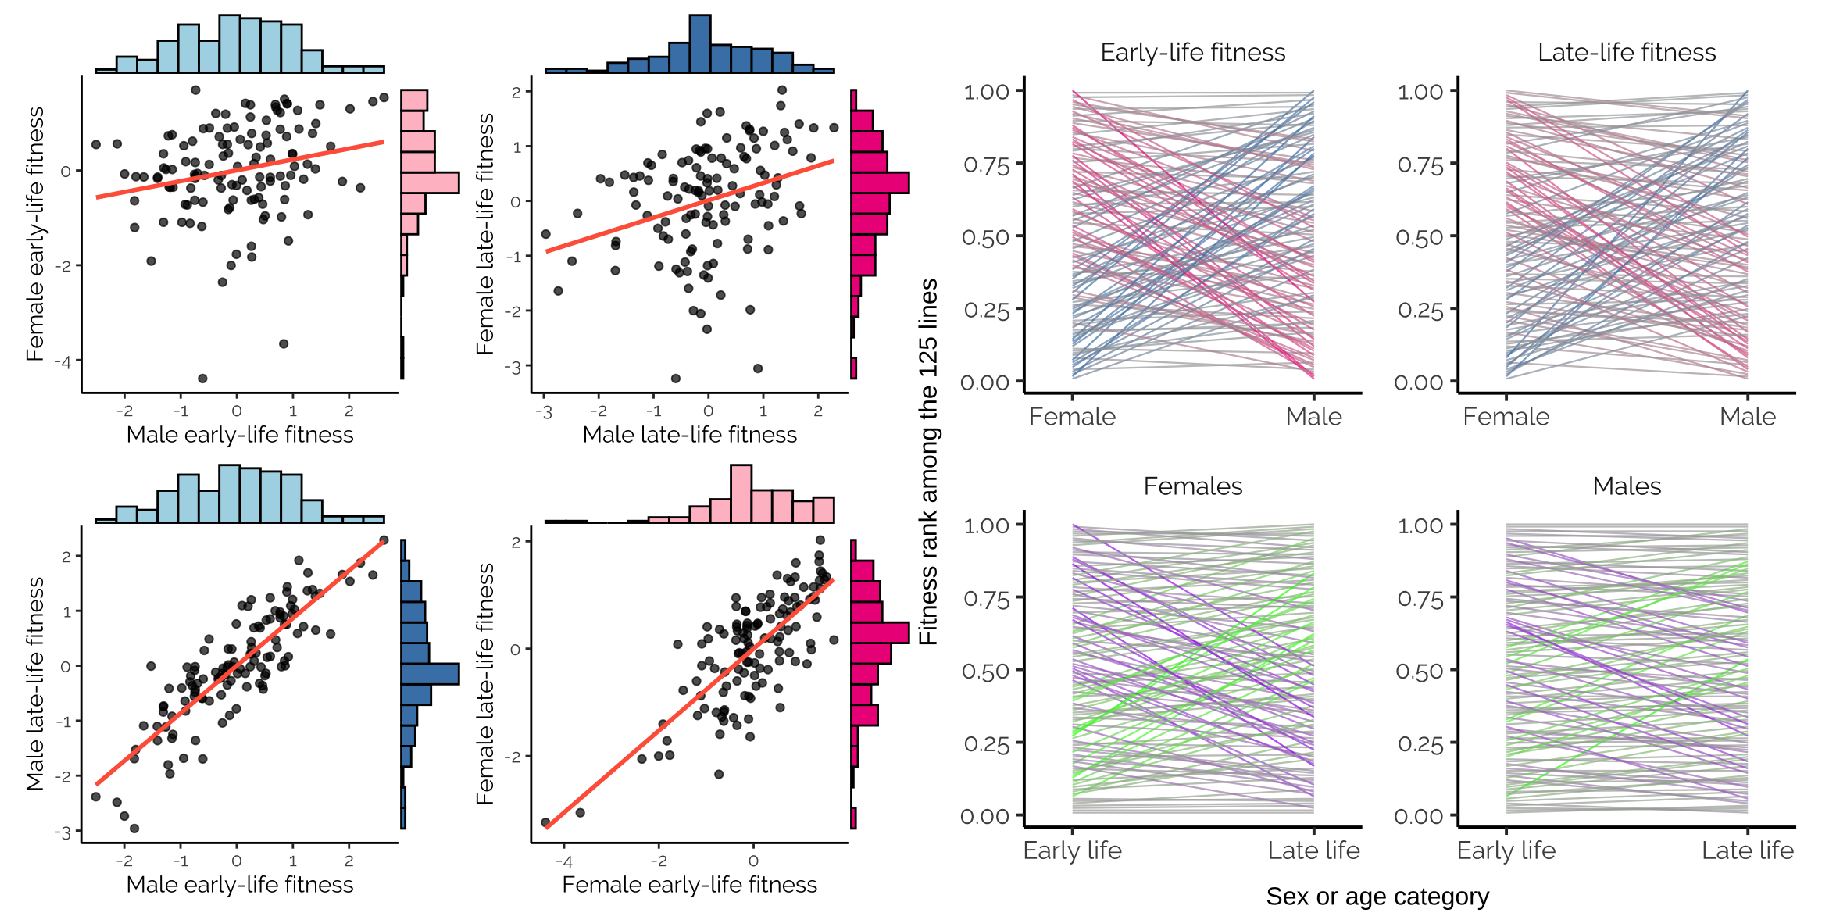
\includegraphics[width=1.0\textwidth]{../figures/fig1.pdf}
\caption{\footnotesize{Panel A shows correlations among estimated line means for the four fitness components from Bayesian mixed models adjusting for block effects. Panel B shows the same data expressed as ranks, and the panels illustrate how the ranks co-vary between pairs of phenotypes (the colours indicate the slope of the line, e.g. redder lines have high-ranked female fitness and low-ranked male fitness).}}
\end{figure}
\newpage

\subsection*{Genetic variance and covariance in fitness}

The estimated G matrix for our four traits is shown in Table 1. Fitness
was highly heritable\ldots{}

\subsection*{Distribution of fitness effects across variants}

Figure 2 plots the mashr-adjusted effect sizes of the polymorphic loci
on each of the four phenotypes (see Table SX for associated Spearman
correlation statistics). As expected based on the line means in Figure
1, there was a positive correlation, such that at loci where the minor
allele increase or decrease female fitness, the minor allele tended to
have a similar effect on male fitness. The correlation was similarly
strong in both age classes, though the slope was shallower in the late
life age class due to a smaller effect sizes on male fitness as compared
to the early life age class.

The mean effect on fitness across all variants was significantly
negative for all but one of the phenotypes, which means that the minor
alleles were, on average, associated with lower fitness than the major
alleles (Table SX). The exception was male early-life fitness, for which
the reverse was true: the major allele tended to be associated with
lower fitness than the minor allele. However the average variant effect
size differed by only a small amount from zero (i.e.~the value expected
under the null hypothesis that the minor and major alleles are equally
likely to be the beneficial one).

\begin{figure}[h]
\centering
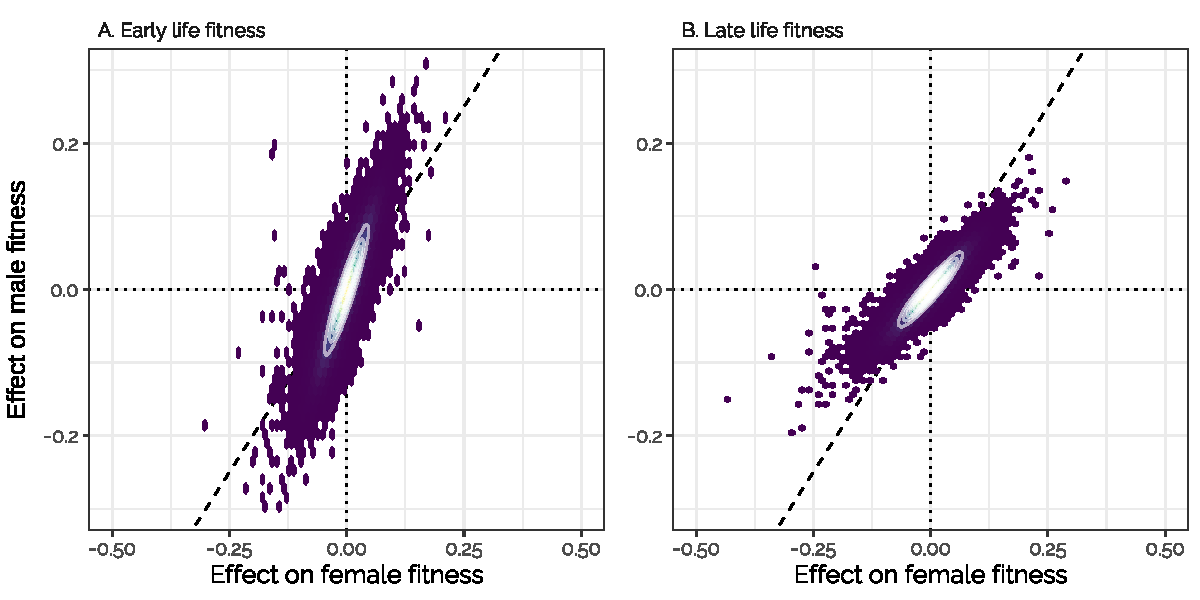
\includegraphics[width=1.0\textwidth]{../figures/SNP_effect_ED.pdf}
\caption{\footnotesize{Effect sizes of 1,207,357 loci (i.e. groups of one or more polymorphic sites in complete linkage disequilibrium) on male and female fitness, plotted separately for the early-life and late-life estimates. The effect sizes estimated using GEMMA have been corrected using mashr, using the data-driven method to apply shrinkage (Figure SX shows the raw estimates). The data have been binned into hexagons, with the colour and contour lines indicating the number of loci. The diagonal line represents $y=x$. Positive effect sizes indicate that the minor allele is associated with higher fitness.}}
\end{figure}
\newpage

\subsection*{Top hits from the GWAS}

We used the SNP clumping method in PLINK to identify groups of loci in
linkage disequilibrium with one another, for which at least one group
member affected one of the four phenotypes with \(-log10(p) > 5\) (Table
SX). There were 83 such groups of loci (15 groups with
\(-log10(p) > 6\), and 3 with \(-log10(p) > 7\)). Many of these regions
overlapped genes. For example, we found a significant variant
(\(-log10(p) = 7.3\)) in an intron of \emph{serontonin receptor 1A}
(FBgn0004168), where the minor allele (MAF = 0.11) reduced fitness in
both sexes. A complete list of affected genes in given in Table SX.

We found one polymorphic region that had a sexually antagonistic effect
on fitness (with the major allele benefitting females and harming males;
MAF = 0.10), overlapped six genes: \emph{Death regulator Nedd2-like
caspase} (\emph{Dronc}; FBgn0026404), \emph{variable nurse cells}
(\emph{vnc}; FBgn0263251), and \emph{defective proboscis extension
response 6} (\emph{dpr6}; FBgn0040823) plus 3 uncharacterised genes
(FBgn0036062, FBgn0036063, and FBgn0259932). \emph{Dronc} mediates
caspase-dependent cell death, and is implicated in the DNA damage
response, sperm differentiation, and cell specification, while
\emph{vnc} is involved in histone acetylation and oogenesis. \emph{dpr6}
is involved in synapse organisation and the perception of chemical
stimuli; another \emph{dpr} gene is required for proper male courtship
(\url{https://journals.plos.org/plosgenetics/article?id=10.1371/journal.pgen.0030216}).
The three uncharacterised genes all show high expression in the ovary
and less expression in the testis (modENCODE Tissue Expression),
implying roles in reproduction.

\subsection*{Top hits from the TWAS}

\subsection*{Almost all loci affect fitness, or are close to a locus that does}

Inspired by Figure 1C in Boyle et al.~(REF), we sorted all of the
variants by their fitness effects, placed them in bins of 1000, and then
calculated the average fitness effect for each bin. Figure 3 shows that
there was a very tight correlation (XXX) between the average effects of
the variants in each bin on male and female fitness, and that the shape
of the relationship was different between age classes. For the early
life age class, there was a very tight positive correlation between the
effect size on males and females for loci where the minor allele
increased fitness in females (i.e.~those \(x > 0\) in Figure 3A). For
loci where the major allele increased female fitness (\(x < 0\) in
Figure 3A), the correlation was non-linear, such that the effect of the
major allele on male fitness became less positive as its effect on
females increased. Figure 3A thus implies a shortage of loci where the
major allele is strongly beneficial to fitness in both sexes in the
early life age class (though there was no shortage of loci where the
minor allele was strongly beneficial in both sexes). Figure 1B showed
similar patterns, except that the relationship did not change between
loci where the minor versus major allele benefitted females.

Figures 3 reaffirms the results shown in Figures 1-2 that there is a
positive genetic correlation between male and female fitness, and that
this correlation changes between age classes, but Figure 3 also implies
that our four phenotypes are highly polygenic (or `omnigenic'; Boyle et
al.~REF) and are affected by large numbers of loci with small effects.
The male and female fitness measurements were collected independently,
and so Figure 3 allows us to distinguish small but genuine effects from
statistical noise, despite the low power of our study (and most GWAS) to
detect variants with weak effects. To see why, consider an alternative
hypothesis, in which the great majority of variants have no effect on
fitness, and the genetic (co)variance in phenotypes observed across
lines (Figure 1 and QUANT GEN TABLE) resulted from comparatively few
(e.g.~dozens) of variants with comparatively large effects. The plot in
Figure 3 would then be flat in the centre with steep inflections at each
end. The straight line that we see instead suggests that there a large
number of variants that each affect fitness - typically in both sexes,
in the same direction - whose effect sizes range from tiny to moderate.
Put another way, the effect size of each 1000-variant bin on female
fitness was replicated for male fitness, suggesting that many of the
non-zero effect size estimates refelct real non-zero effects, as opposed
to statistical sampling variance.

\begin{figure}[h]
\centering
\includegraphics[width=1.0\textwidth]{../figures/boyle_plot.pdf}
\caption{\footnotesize{Mean effect size on each phenotype for groups of 1,000 loci. The loci were first sorted in order of their effect on female fitness, then binned and their effect sizes on each sex were calculated. The line shows a quadratic linear regression fit with standard error in grey.}}
\end{figure}
\newpage

\subsection*{Mixture modelling results from the GWAS and TWAS}

Figure 4A shows the results of a mixture modelling analysis of the GWAS
results, from the R package \texttt{mashr} (in canonical mode).
\texttt{mashr} allows one to estimate the proportions of various types
of locus, using a set of covariance matrices (\(4\times4\) matrices, in
our case) that are specified \emph{a priori} by the user. To be
inclusive of all possibilities, we hypothesised that loci might A) have
no effect on any of the four phenotypes, B) affect one of the four
phenotypes and not the others, C) affect both phenotypes for one sex,
either concordantly or antagonistically across age classes, D) affect
both phenotypes for one age class, either concordantly or
antagonistically across sexes, or E) affect all four phenotypes in the
same direction or differing directions (including complex types, such as
loci that are sexually antagonistic in one age class and sexually
concordant in the other). Several of these possibilities were calculated
to apply to fewer than 1\% of loci by \texttt{mashr}, and thus are not
plotted in Figure 4. We ran \texttt{mashr} once for all the loci, and
ran it a further 5 times using just the loci from one of the 5 major
chromosome arms.

Figure 4A shows that the most common type of locus was estimated to be
the type that has an identical effect size on all four phenotypes
(recorded as `sexually concordant' in Figure 4A). The model estimated
that 0\% of loci have age-specific or age-antagonistic effects, and so
these types are not plotted. Loci with no effect on fitness were rare,
despite the model's prior that this type of locus is ten-fold more
common than any other type, again indicating that most loci either
affect fitness or are closely linked to a locus that does. Loci with
sex-specific effects were estimated to be quite common, especially loci
with sexually antagonistic (12\%, genome-wide) or female-specific
effects (19\%). The X chromosome was inferred to have the highest
proportion of sexually antagonistic loci (24\%), with an estimate that
was twice as high as the estimate for the whole genome, and
substantially higher than for other chromosomes (e.g.~7.4\% for
chromosome 2L).

\subsection*{Distribution of fitness effects across chromosomes}

To do\ldots{}

\section*{Discussion}

\newpage
\section*{Tables}

\textbf{Table 1}: List of variables, and their corresponding
parameter(s) in the model, which were varied in order to study their
effects on extinction. \#
\texttt{\{r\ xtable,\ results="asis"\}\ \#\ print\_table1()\ \#}

\newpage
\section*{Figures}

\bibliographystyle{unsrt}
\bibliography{references.bib}


\end{document}
